%! TeX root = main.tex
\documentclass[a4paper]{article}
\title{Linear Feedback Shift Registers} 
\author{Angelo Panariti}
\usepackage{circuitikz}
\usepackage{tikz-timing}
\usepackage{hyperref}
\begin{document}
\maketitle
\centerofcontents
\section{Introduction to Linear Feedback Shift Registers}

\begin{itemize}
    \item
        Goal: Stream ciphers that is small and low power in hardware.
    \item
        Example: A5-1 Cipher in GSM
        \begin{itemize}
            \item
                consists of 3 LFSRs
        \end{itemize}
\end{itemize}

Atomic elements: flip-flop, stores a single bit


\centering
\begin{circuitikz}
   \node[flipflop D](D1){};
\end{circuitikz}

Clock input (determines when the bit is to be stored or not depending on the input signal).

Let's try to build a PRNG. Connect 3 flip-flops $(1,0,0)$. We generate a clock pulse.

\centering
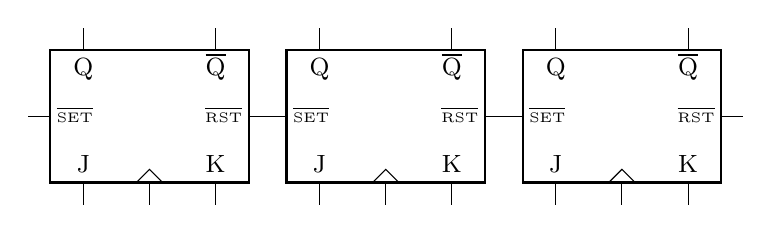
\begin{tikzpicture}
\draw (3,0) node[flipflop JK, add async SR, rotate=90]{};
\draw (6,0) node[flipflop JK, add async SR, rotate=90]{};
\draw (9,0) node[flipflop JK, add async SR, rotate=90]{};
\end{tikzpicture}
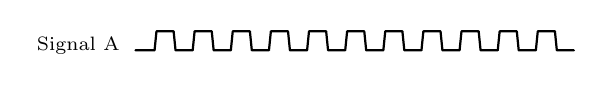
\begin{tikzpicture}[timing/picture, thick]
    \node[anchor=base, font=\scriptsize] at (-3,2) {Signal A};
    \timing at (0,2) {LHLHLHLHLHLHLHLHLHLHLHL};
\end{tikzpicture}
\begin{table}
\centering
    \begin{tabular}{|c|c|c|}
        \hline
        1 & 0 & 0 \\
        \hline
        0 & 1 & 0 \\
        \hline
        1 & 0 & 1 \\
        \hline
        1 & 1 & 0 \\
        \hline
        1 & 1 & 1 \\
        \hline
        0 & 1 & 1 \\
        \hline
        0 & 0 & 1 \\
        \hline
        1 & 0 & 0 \\
        \hline
    \end{tabular}
\end{table}

\

\subsection{Mathematical description}
We run into a cycle after group of 7 output bits ($S_0, S_1, S_2, ..., S_7$). 


$$S_3 \equiv S_1+S_0 \ mod \ 2$$
$$S_4 \equiv S_2+S_1 \ mod \ 2$$
$$S_{i+3} \equiv S_{i+1}+S_i \ mod \ 2$$

\

Instead of a period of length 7 bits, we would need a few billion/trillion bits and then it starts to repeat.

\section{General LFSRs}

$m$ numbers of flip-flops. Every flip-flop becomes a switch. 
We introduce a multiplier that acts like a switch

\

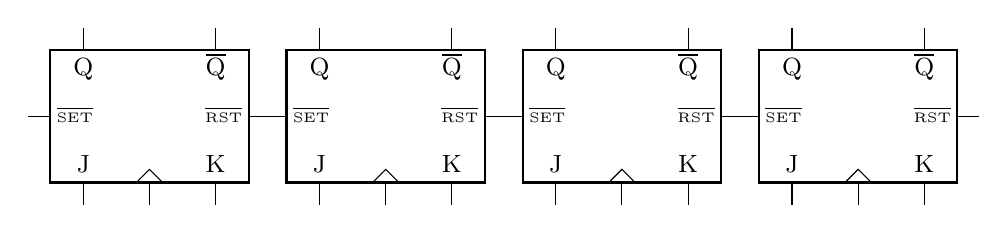
\begin{tikzpicture}
\draw (3,0) node[flipflop JK, add async SR, rotate=90]{};
\draw (6,0) node[flipflop JK, add async SR, rotate=90]{};
\draw (9,0) node[flipflop JK, add async SR, rotate=90]{};
\draw (12,0) node[flipflop JK, add async SR, rotate=90]{};
\end{tikzpicture}
\
$$ A \rightarrow [X] \rightarrow B$$
$$P_i = 1, B=p_i, A = A$$
$$P_i = \emptyset, B=p_i, A=\emptyset $$
$$S_m \equiv S_{m-1}P_{m-1} + S_{m-2}P_{m-2} + ... + S_1P_1 + S_0P_0 \ mod \ 2$$
$$S_{m+1} \equiv S_{m}P_{m-1} + S_{m-1}P_{m-2} + ... + S_2P_1 + S_1P_0 \ mod \ 2$$

\
\

\noindent\fbox{\begin{minipage}{\dimexpr\textwidth+1\fboxsep-500\fboxrule\relax}

\subsection{Equation}
\label{marker}
$$S_{m+1} = \sum_{i=0}^{m-1} S_{i+j} \cdot P_{j} \ mod 2$$

$$i = 0,1,2,3 $$

\
\end{minipage}}

\

\noindent\fbox{\begin{minipage}{\dimexpr\textwidth+1\fboxsep-500\fboxrule\relax}
\subsection{Theorem}

The maximum period (or sequence length) generated by an LFSR is $2^m - 1$.
\end{minipage}}

\

\noindent\fbox{\begin{minipage}{\dimexpr\textwidth+1\fboxsep-500\fboxrule\relax}
        \subsection{Theorem }
Only certain feedback configurations ($p_{m-1},..., p_0$) yield maximum length sequences
\end{minipage}}


m = flip-flops, 0 open, 1 close

\

Ex: $m =4, \ \ p_3=p_2=0,\ p_1=p_0 = 1$


\

Ex: $m =4, \ \ p_3=p_2=p_1=p_0 = 1$


\subsection{Notation}

LFSRs are often specified by the polynomial

$$P(x) = x^m + p_{m-1} x^{m-1} + ... + p_1 x + p_0$$

Only LFSRs with primitive polynomials yield maximum length sequences.



\section{Attacks against single LFSRs}


Given:

    - all $y_i$

    - degree $m$

    - $x_0,...,x_{2m-1}$

\begin{enumerate}
    \item First step

$$y_i \equiv x_i + s_i \ mod \ 2$$
$$s_i \equiv y_i + x_i \ mod \ 2$$

\item Second step

    Goal: recover S_{2m},S_{2m+1},S_{2m+2},...

    Q: What is $p_0, p_1,...,p_{m-1}$?

    Using what we mentioned in \nameref{marker} [2.1], we can solve for 

    $$S_m \equiv S_{m-1}P_{m-1} +  ... + S_0P_0 \ mod \ 2$$
    $$S_{m+1} = S_m p_{m-1} + ...  + S_1p_0 mod 2$$
    $$S_{2m+1} = S_{2m-2} p_{m-1} + ... + S_{m-1}p_0 \ mod 2$$

System of m linear equations with m unknowns. $\rightarrow$ can easily be solved with Gaussian elimination (or matrix inversion). If an attacker knows (at least) $2m$ output values of an LFSR, he can recover the entire LFSR configuration.

\item Third step

- Using $(p_{m-1},...,p_0)$ build LFSR

- compute $s_0,...,s_{2m-1},s_{2m},s_{2m+1}...$

- decipher


$$ x_i \equiv y_i + s_i \ mod \ 2$$
\end{enumerate}
\end{document}
